% !Mode:: "TeX:UTF-8"

\chapter{绪论\label{intro}}


\section{研究背景与意义}

引用参考文献例子 \cite{USE} \cite{USE2}

特殊字符:
\textbf{粗体}
\emph{斜体}
$alphagraph$

空~格,$\lambda$,$\epsilon$  $\in$

分点:
\begin{enumerate}
	\item{} 无标题
	\item{分点2标题}
	\item 3333
\end{enumerate}

公式:
\begin{equation}
u_{i,j,G} =\left\{
   \begin{array}{ll}
   v_{i,j,G}, & \forall j = {\langle l \rangle}_{D},{\langle l+1 \rangle}_{D},\ldots,{\langle l+L-1 \rangle}_{D} \\
   x_{i,j,G}, & {\rm otherwise} \
   \end{array}\right.,
\label{EX}
\end{equation}

\begin{equation}
u_{i,j,G} =\left\{
   \begin{array}{ll}
   v_{i,j,G}, &\ {\rm if} \  rand_{j}(0,1) \le DD \; or \; j=j_{rand} \\
   x_{i,j,G}, &\ {\rm otherwise} \
   \end{array}\right.,
\label{DEX}
\end{equation}

\begin{equation}
{\rm PCD}(x^i,x^j)=
\begin{cases}
0.5 & {\rm if}\ \forall m, L_m^i=L_m^j \\
\sum_{m=1}^{M}|L_m^i-L_m^j| & {\rm otherwise} \\
\end{cases}
.
\end{equation}


算法流程:
\begin{algorithm}[t] %[]里面设置样式,[tp],[!tp]等
\footnotesize
\caption{算法名字}
\label{algo_CCMODE_CCM}
set generation $t=0$;
\tcc*{Initialization}
\For {each cahahah $m=1$ to $M$}
{
	\For{each $i=1$ to $NP$ }
	{
		randomly  \;
		 $X_{i}^{m}$,
	}
}
\While {stopping criterion is not met}
{
	\While {$AlalalalA$}
	{
		distance-ae\;
		$A = A \cup \mathcal{F}_{i}$,
		$i=i+1$\;
	}
}
\end{algorithm}

插入图片:

\begin{figure*}[ht]
\centering
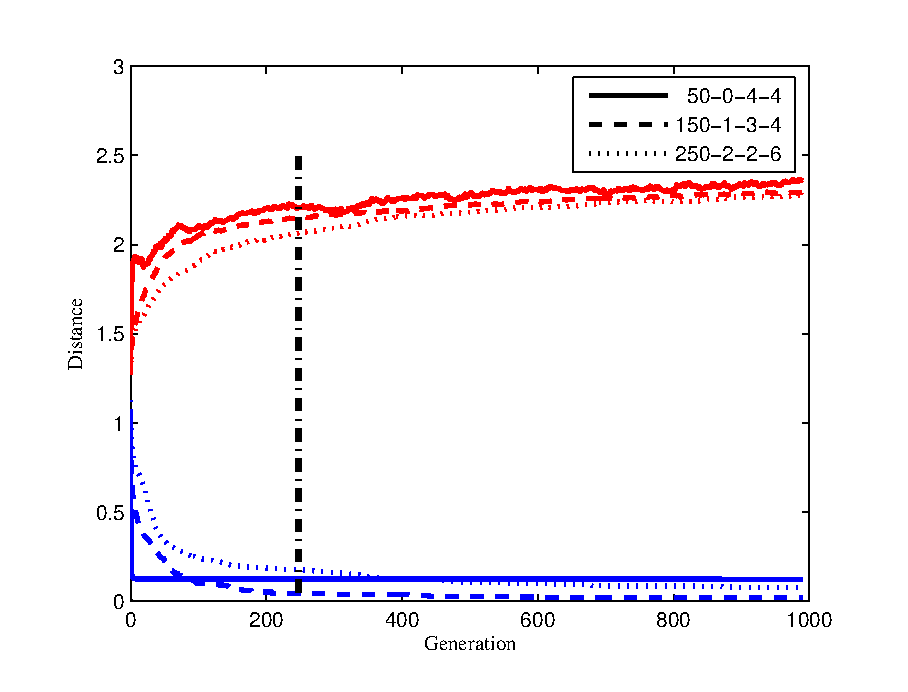
\includegraphics[height=4cm]{figures/parameter.eps}
\caption{标题}
\label{labeliiiiii}
\end{figure*}


\begin{table}
%\tiny 放不下把表格缩小
\centering
\caption{表名}
\label{tab:1}
% Table generated by Excel2LaTeX from sheet 'wilcoxon test4'
\begin{tabular}{l|c|c|c|c|c}
\hline
$11$    & $111$      & $11$+         & $11$-         & 11    & $\alpha$ = 0.05   \\
\hline
1 & 1/2& 458.0 & 70.0 & 1.2158E-4 & Y11ES \\ \hline
1& 301/1& 518.0 & 10.0 & 2.002E-8 & YE11S \\ \hline
1 & 11/8& 308.0 & 220.0 & $\geq$ 0.2 & 1NO \\ \hline
1 & 21/1& 518.0 & 10.0 & 2.002E-8 & YE111S \\ \hline
\hline

\end{tabular}%
\end{table}


\section{研究现状}

\section{本文工作}

\section{论文结构}
